\documentclass[AMA,twocolumn]{USG}
\usepackage{xcolor}
\usepackage{minted}
\usemintedstyle{trac}
\setminted{linenos=true, fontsize=\footnotesize}

\definecolor{LightGray}{gray}{0.9}

\articletype{Undertale in Extremis: Simulador de Batalhas em Risc-V}

\begin{document}

\title{Trabalho de Organização de Computadores}

\author[1]{João Luís Almeida Santos}

\address[1]{\orgname{Universidade Federal da Fronteira Sul,}%
\orgaddress{\city{Chapecó}, \state{Santa Catarina}, \country{Brasil}}}

\maketitle

\section{Introdução}
\begin{figure}[h]
\centering
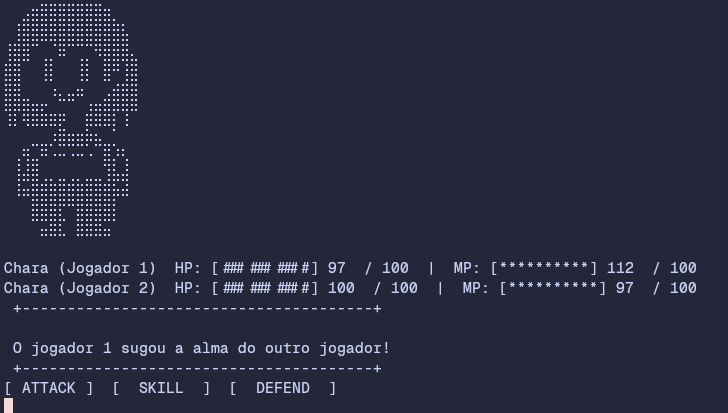
\includegraphics[width=\linewidth]{images/jogo.png}
\caption{Interface do simulador de batalhas no modo de observação.}\label{fig:jogo}
\end{figure}

O presente projeto documenta a tentativa de criar um simulador de batalhas de RPG, no estilo Pokémon (Figura~\ref{fig:jogo}),
dentro do ambiente RISC-V, utilizando o RARS como ferramenta de simulação. A ISA utilizada é a
RISC-V RV32IM, isto é, um conjunto de instruções que contempla apenas operações com inteiros,
além de instruções de multiplicação e divisão.
\\\\
O projeto, denominado \textit{Undertale in Extremis}, foi desenvolvido como proposta alternativa 
às opções listadas na comanda, com autorização do professor.
 O sistema simula batalhas entre dois bots autônomos que se enfrentam em 
 turnos até que um deles seja eliminado. Cada bot recebe uma estratégia e age por conta própria, 
 escolhendo a cada turno entre seis ações: ataque, defesa, Absolute Grit, Soul Suck, Final Execution e Mirror Shield.
 Ambos os bots iniciam com 100 pontos de vida (HP) e 100 de mana (MP), sendo o MP regenerado em +2 por turno.
\\\\
\begin{table}[h]
\caption{Ações disponíveis por turno}
{\renewcommand{\arraystretch}{1.5}
\begin{tabular}{p{1.8cm}p{4.5cm}p{1.2cm}}
\hline
\textbf{Ação} & \textbf{Efeito} & \textbf{Custo} \\
\hline
Ataque         & 1d20: erro $<$10, hit $\geq$10, dúplica o dano em 20. & 0 MP \\
Defesa         & Bloqueia o próximo ataque. Contra-ataca quando crítico. & 0 MP \\
Absolute Grit  & Garante um crítico. & 20 MP \\
Soul Suck      & 1--12 de auto-dano; ganha 4$\times$ em MP. & 0 MP \\
Final Execution & 800\% de dano. Falha se alvo $>$50\% HP. & 150 MP \\
Mirror Shield  & Reflete o próximo ataque recebido. & 30 MP \\
\hline
\end{tabular}}
\end{table}

O ataque realiza uma verificação 1d20: abaixo de 10 erra, acima acerta, e no 20 resulta em crítico com dano dobrado.
A defesa bloqueia o próximo ataque recebido, podendo ripostar em um crítico.
A Absolute Grit garante um crítico ao custo de 20 MP.
A Soul Suck causa 1--12 de dano ao próprio bot, drenando igual MP do inimigo e ganhando 4$\times$ esse valor, podendo ultrapassar o limite de 100 MP.
A Final Execution causa 800\% de dano ao custo de 150 MP, mas falha se o alvo estiver acima de 50\% de HP.
O Mirror Shield reflete o próximo ataque recebido de volta ao atacante, ao custo de 30 MP.

\begin{table}[h]
\caption{Atributos iniciais de cada bot}
{\renewcommand{\arraystretch}{1.5}
\begin{tabular}{ll}
\hline
\textbf{Atributo} & \textbf{Valor} \\
\hline
HP & 100 \\
MP & 100 \\
Regeneração de MP & +2 por turno \\
\hline
\end{tabular}}
\end{table}


\begin{table}[h]
\caption{Estratégias dos bots}
{\renewcommand{\arraystretch}{1.5}
\begin{tabular}{p{1.2cm}p{1.4cm}p{4.5cm}}
\hline
\textbf{Bot} & \textbf{Estratégia} & \textbf{Comportamento} \\
\hline
Flowey & Aleatório  & Escolhe uma das seis ações por RNG a cada turno, sem avaliar estado algum. \\
Chara  & Inteligente & Acumula MP via Soul Suck até atingir 150 MP, reduz o inimigo abaixo de 50\% de HP com Absolute Grit e então dispara a Final Execution. \\
Toby   & Troll    & Monitora o próprio HP e o MP do inimigo. Se estiver abaixo de 50 HP e o inimigo tiver $\geq$150 MP, levanta o Mirror Shield para refletir a Final Execution. Fora dessa janela, mistura ataques e Soul Suck, e executa o inimigo quando as condições permitem. \\
\hline
\end{tabular}}
\end{table}

\section{Desafios e Soluções}

\subsection{Gerenciamento de Stack}

O programa usa macros para abstrair e automatizar as operações necessárias de gerenciamento da stack
durante chamadas de função. Essa estratégia facilitou o desenvolvimento e reduziu a ocorrência de erros
relacionados ao gerenciamento da stack. O código apresentado corresponde a uma versão compatível apenas 
com o RARS, visto que, em outros \textit{assemblers}, utiliza-se a diretiva \texttt{.endm} 
em vez de \texttt{.end\_macro}. Aprendi essa técnica no último semestre de ORG.
\\\\

\begin{minted}{asm}
    .macro     startF
    addi       sp, sp, -20
    sw         ra, 16(sp)
    sw         s0, 12(sp)
    sw         s1, 8(sp)
    sw         s2, 4(sp)
    sw         s3, 0(sp)
    .end_macro

    .macro     endF
    lw         ra, 16(sp)
    lw         s0, 12(sp)
    lw         s1, 8(sp)
    lw         s2, 4(sp)
    lw         s3, 0(sp)
    addi       sp, sp, 20
    .end_macro

\end{minted}

\section{Conclusão}

\section{Anexos}

\end{document}
